% formal/sat.tex
% SPDX-License-Identifier: CC-BY-SA-3.0

\section{SAT Solvers}
\label{sec:formal:SAT Solvers}

제한된 횟수의 루프와 재귀를 갖는 모든 유한한 프로그램은 입력에 대한 그
프로그램의 단정들을 표현하는 논리 표현식으로 변환될 수 있습니다.
그런 논리 표현식이 있다면, 어떤 입력의 조합이 단정문 가운데 하나를 터지게 만들
수 있는지 알 수 있는지 여부를 아는 것은 매우 흥미로울 겁니다.
만약 입력이 이진 변수들의 조합으로 표시된다면, 이는 곧 satisfiability problem
이라고도 알려진 SAT 입니다.
SAT solver 들은 하드웨어의 검증에서 많이 사용되어져 왔으며, 여기서 커다란
진보의 동기를 주었습니다.
1990년대 초의 월드 클래스 SAT solver 는 100 개의 별개의 이진 변수들로 표현된
논리 표현식을 다룰 수 있습니다만, 2010년대 초에 와서는 백만개의 변수로 이루어진
SAT solver 들이 사용 가능합니다~\cite{Kroening:2008:DPA:1391237}.
\iffalse

Any finite program with bounded loops and recursion can be converted
into a logic expression, which might express that program's assertions
in terms of its inputs.
Given such a logic expression, it would be quite interesting to know
whether any possible combinations of inputs could result in one of
the assertions triggering.
If the inputs are expressed as combinations of boolean variables,
this is simply SAT, also known as the satisfiability problem.
SAT solvers are heavily used in verification of hardware, which has
motivated great advances.
A world-class early 1990s SAT solver might be able to handle a logic
expression with 100 distinct boolean variables, but by the early 2010s
million-variable SAT solvers were readily
available~\cite{Kroening:2008:DPA:1391237}.
\fi

또한, SAT solver 들을 위한 프론트 엔드 프로그램들은 C 코드를 자동으로 논리
표현식으로 변환시킬 수 있으며, 이 때 단정문들을 취하기도 하고 배열 크기 침범
에러들과 같은 에러 조건들을 위한 단정문을 생성하기도 합니다.
한가지 예는 C bounded model checker, 또는 \co{cbmc} 라 알려진 것으로, 많은
리눅스 배포판에 포함되어 있어서 사용 가능합니다.
이 도구는 사용하기가 상당히 간단해서, \co{cbmc test.c} 만으로도 \path{test.c}
를 검증하기에 충분합니다.
이런 사용상의 편의성은 회귀 테스트 프레임워크에 포함되고 있는 형식적 검증으로의
문을 열어주기 때문에 매우 중요합니다.
대조적으로, 특정 목적의 언어로의 사소하지 않은 변환을 필요로 하는 전통적인
도구들은 설계 시점에서의 검증으로만 국한되어졌습니다.
\iffalse

\begin{figure}[tbp]
\centering
\resizebox{2in}{!}{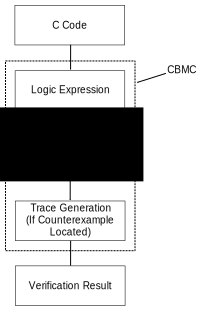
\includegraphics{formal/cbmc}}
\caption{CBMC Processing Flow}
\label{fig:formal:CBMC Processing Flow}
\end{figure}

In addition, front-end programs for SAT solvers can automatically translate
C code into logic expressions, taking assertions into account and generating
assertions for error conditions such as array-bounds errors.
One example is the C bounded model checker, or \co{cbmc}, which is
available as part of many Linux distributions.
This tool is quite easy to use, with \co{cbmc test.c} sufficing to
validate \path{test.c}, resulting in the processing flow shown in
Figure~\ref{fig:formal:CBMC Processing Flow}.
This ease of use is exceedingly important because it opens the door
to formal verification being incorporated into regression-testing
frameworks.
In contrast, the traditional tools that require non-trivial translation
to a special-purpose language are confined to design-time verification.
\fi

근래에 들어서, SAT solver 들은 병렬 코드를 처리하는 형태로도 나타났습니다.
이런 solver 들은 입력이 되는 코드를 single static assignment (SSA) 형태로
변환시키고는 여기서 생겨날 수 있는 모든 액세스 순서들을 생성합니다.
이 방법은 잘 동작할 듯 보입니다만, 실제 환경에서 얼마나 잘 동작할지는 볼 필요가
있습니다.
한가지 좋은 징조는 2016년에 있었던 \co{cbmc} 를 리눅스 커널 RCU 에 적용하려 한
작업~\cite{LihaoLiang2016VerifyTreeRCU,LanceRoy2017CBMC-SRCU} 입니다.
이 작업은 RCU 의 최소한의 구성과 작은 수의 쓰레드를 사용한 검증 시나리오를
사용하긴 했습니다만, 리눅스 커널 C 코드를 수집하고 유용한 결과를 내놓았습니다.
이 C 코드에서 생성된 논리 표현식은 9천만개의 변수, 4만5천개의 절들을 가져서 이
SAT solver 가 올바른 결과를 내놓는데 수십기가바이트의 메모리 사용과 80시간의
CPU 시간을 필요로 했습니다.
\iffalse

More recently, SAT solvers have appeared that handle parallel code.
These solvers operate by converting the input code into single static
assignment (SSA) form, then generating all permitted access orders.
This approach seems promising, but it remains to be seen how well
it works in practice.
One encouraging sign is work in 2016 applying \co{cbmc} to Linux-kernel
RCU~\cite{LihaoLiang2016VerifyTreeRCU,LanceRoy2017CBMC-SRCU}.
This work used minimal configurations of RCU, and verified scenarios
using small numbers of threads, but nevertheless successfully ingested
Linux-kernel C code and produced a useful result.
The logic expressions generated from the C code had up to 90~million
variables, 450~million clauses, occupied tens of gigabytes of memory,
and required up to 80~hours of CPU time for the SAT solver to produce
the correct result.
\fi

그러나, 리눅스 커널 해커는 자신의 코드가 자동으로 검증되었다는 데 대해 회의감을
느낄 수도 있을 것이고, 그런 해커들은 수십년전부터의 많은 그런 회의감을 찾을
겁니다~\cite{DeMillo:1979:SPP:359104.359106}.
그런 비판적 감정을 생산적으로 표현하는 한가지 방법은, 그렇게 검증된 코드의
버그가 삽입된 버전을 제공하는 겁니다.
만약 formal-verification tool 이 모든 버그를 찾는다면, 우리의 해커는 이 도구의
기능에 대해 더 만족할 수 있을 겁니다.
그리고 이게 바로 리눅스 커널 RCU 에 버그가 잠재적으로 삽입되어 있는 20개의 서로
다른 브랜치를 갖는 \co{git}
저장소~\cite{PaulEMcKenney2017VerificationChallenge6}를 가진 이유입니다.

현재, \co{cbmc} 는 여러개의 주입된 버그들을 찾을 수 있습니다만, RCU 의
메인테이너가 아직 알지 못한 버그를 찾지는 못했습니다.
그러나, SAT solver 들이 언젠가는 병렬 코드의 동시성 버그를 찾는데 유용해질 날이
올거라는 희망을 가질만 합니다.
\iffalse

Nevertheless, a Linux-kernel hacker might be justified in feeling skeptical
of a claim that his or her code had been automatically verified, and
such hackers would find many fellow skeptics going back
decades~\cite{DeMillo:1979:SPP:359104.359106}.
One way to productively express such skepticism is to provide bug-injected
versions of the allegedly verified code.
If the formal-verification tool finds all the injected bugs, our hacker
might gain more confidence in the tool's capabilities.
Of course, tools that find valid bugs of which the hacker was not yet aware
will likely engender even more confidence.
And this is exactly why there is a \co{git} archive with a 20-branch set
of mutations, with each branch potentially containing a bug injected
into Linux-kernel RCU~\cite{PaulEMcKenney2017VerificationChallenge6}.
Anyone with a formal-verification tool is cordially invited to try that
tool out on this set of verification challenges.

Currently, \co{cbmc} is able to find a number of injected bugs,
however, it has not yet been able to locate a bug that RCU's
maintainer was not already aware of.
Nevertheless, there is some reason to hope that SAT solvers will someday
be useful for finding concurrency bugs in parallel code.
\fi
